\subsection{ETSI MEC} 
ETSI (European Telecommunications Standards Institute) on eurooppalainen telealan standardointijärjestö.
ETSI on aloittanut reunalaskennan arkkitehtuurin sekä sen touteuttamiseksi vaadittavien toimintojen määrittelytyön.

ETSI:n MEC spesifikaatio määrittelee reunapalvelun tuottamiseksi vaadittavat ominaisuudet, jotka reunajärjestelmän tulee toteuttaa.
Spesifikaatio listaa myös mahdollisia, mutta ei vaadittuja toimintoja. 
Listaamalla vaaditut toiminnot stanrardi pyrkii yhtenäistämään reunalaskennan konsepteja.  

\subsubsection{Vaatimukset} \label{etsi}
Vaatimukset on jaettu kategorioihin sen mukaan, millaiseen toiminnallisuuteen vaatimus liittyy.
Vaatimuksien kategoriat ovat yleiset vaatimukset (generic requirements), palvelu vaatimukset (service requirements), hallinta vaatimukset (operation and management requirements) ja viimeisenä kategoriana on kokoelma vaatimuksista, joiden teemoina ovat turvallisuus, sääntely ja veloitus (Security, regulation, charging requirements)\cite{etsitechreq}. 

Vaatimukset ovat luonteelta korkean tason kuvauksia reunajärjestelmän toiminnallisuuksista. Yleiset vaatimukset kategorisoitu seuraaviin luokkiin: viitemallin vaatimukset (requirements on the framework), reunapalvelun sovelluksien elinkaari (application lifecycle),
reunapalvelun sovellusympäristö (application enviroment) sekä liikkuvuuden tuki (support of mobility).
Reunajärjestelmän tulee vaatimuksien mukaan pyrkiä hyödyntämään ja tukemaan NFV ratkaisuja hallinnollisten toimien toteuttamiseen.
Vaatimuksien mukaan reunapalvelu tulee voida sijoittaa minne tahansa mobiiliverkon hierarkiassa, esimerkiksi tukiaseman yhteyteen tai EPC:n yhteyteen.
Sijainnin vapaus myös tarkoittaa että reuna-alusta ei voi olla riippuvainen kovin riippuvainen mobiiliverkosta. 
Reunapalvelun sovelluksien elinkaareen liittyvät vaatimukset koskevat pääasiassa reunapalvelun toimijoiden oikeuksia päättää reunan sovelluksien käynnistämisestä ja sulkemista.
Reunapalveluiden sovellusympäristöä koskevissa vaatimuksissa esitetään, että sovelluksien autenttisuus ja eheys täytyy pystyä varmentamaan. Sovellusympäristön täytyy mahdollistaa reunasovelluksen käyttöönotto toisella reunasolmulla \cite{etsitechreq}.
Käytännössä cloudlettienkin yhteydessä esitetty reunalaskennan tuottaminen virtuaalikoneilla mahdollistaisi tämän. 
Mobiiliverkkojen ollessa kyseessä, asiakaslaitteiden liikkuminen tukiasemalta toiselle on keskeinen käyttötapaus. Tämä heijastuu myös vaatimukseen liikkuvuuden tukemisesta reunapalveluissa.
Vaatimuksena on että asiakaslaitteen ja reunapalvelun välisen yhteyden tulee säilyä, vaikka asiakaslaite siirtyisi solusta toiseen tai asiakaslaite siirtyisi sellaiseen soluun, joka on toisen reunasolmun vastuualuetta.

Palveluvaatimukset ovat joukko vaatimuksia, jotka keskittyvät takaamaan reunajärjestelmän perimmäiset palveluperiaatteet.
Lista palveluvaatimuksista on pitkä, joten tähän tutkielmaan on poimittu ainoastaan osa vaatimuksista. Täydellinen lista löytyy \cite{etsitechreq} julkaisusta.
Palveluvaatimukset kuvaavat toiminnallisuuksia, joiden avulla reunapalveluita voidaan tuottaa. 
Tällaisesta esimerkkinä tietoliikenteen reitittämiseen liittyvät vaatimukset, joiden keskeinen tehtävä on kuvata mahdolliset tietoliikennereitit reunapalveluun ja ulos reunapalvelusta.
Yksi, ehkä keskisimmistä, palveluvaatimuksista on reuna-alusta mahdollisuus suodattaa ja muokata verkkoliikennettä. 
Lisäksi kuvataan että reunapalveluiden toimintaa ei haluta rajoittaa pelkästään asiakas-palvelu tyyppisen toimintamalliin. Reunapalveluiden tuottamiselle onkin annettu mikropalvelu -tyyppinen (microservice) kuvaus, jossa palveluntuottajat voivat toimia myös toisten reunapalveluiden kuluttajana.

\subsubsection{Viitekehys ja referenssiarkkitehtuuri}

ETSI:n esittämän viitekehys esittää reunalaskentaan liittyvät korkean tason entiteetit \cite{etsirefarch}. Nämä entiteetit on jaettu kolmeen tasoon: järjestelmä, reunsolmu ja verkko (system, host ja network).
Kuvassa \ref{fig:etsiframework} esitetty kunkin tason entiteetit.
Verkkokerros sisältää verkkoyhteyksistä vastaavat entiteetit. MEC:n tapauksessa verkkokerros koostuu ainakin kolmesta osasta: sisäverkko, ulkoverkko ja mobiiliverkko.
Isäntäkerros koostuu reunapalveluiden virtualisointiin ja reunapalvelun hallinointiin keskittyvistä entiteeteistä.
Järjestelmäkerros koostuu korkeamman tason hallinnosta vastaavista elementeistä.

\begin{figure}[tb]

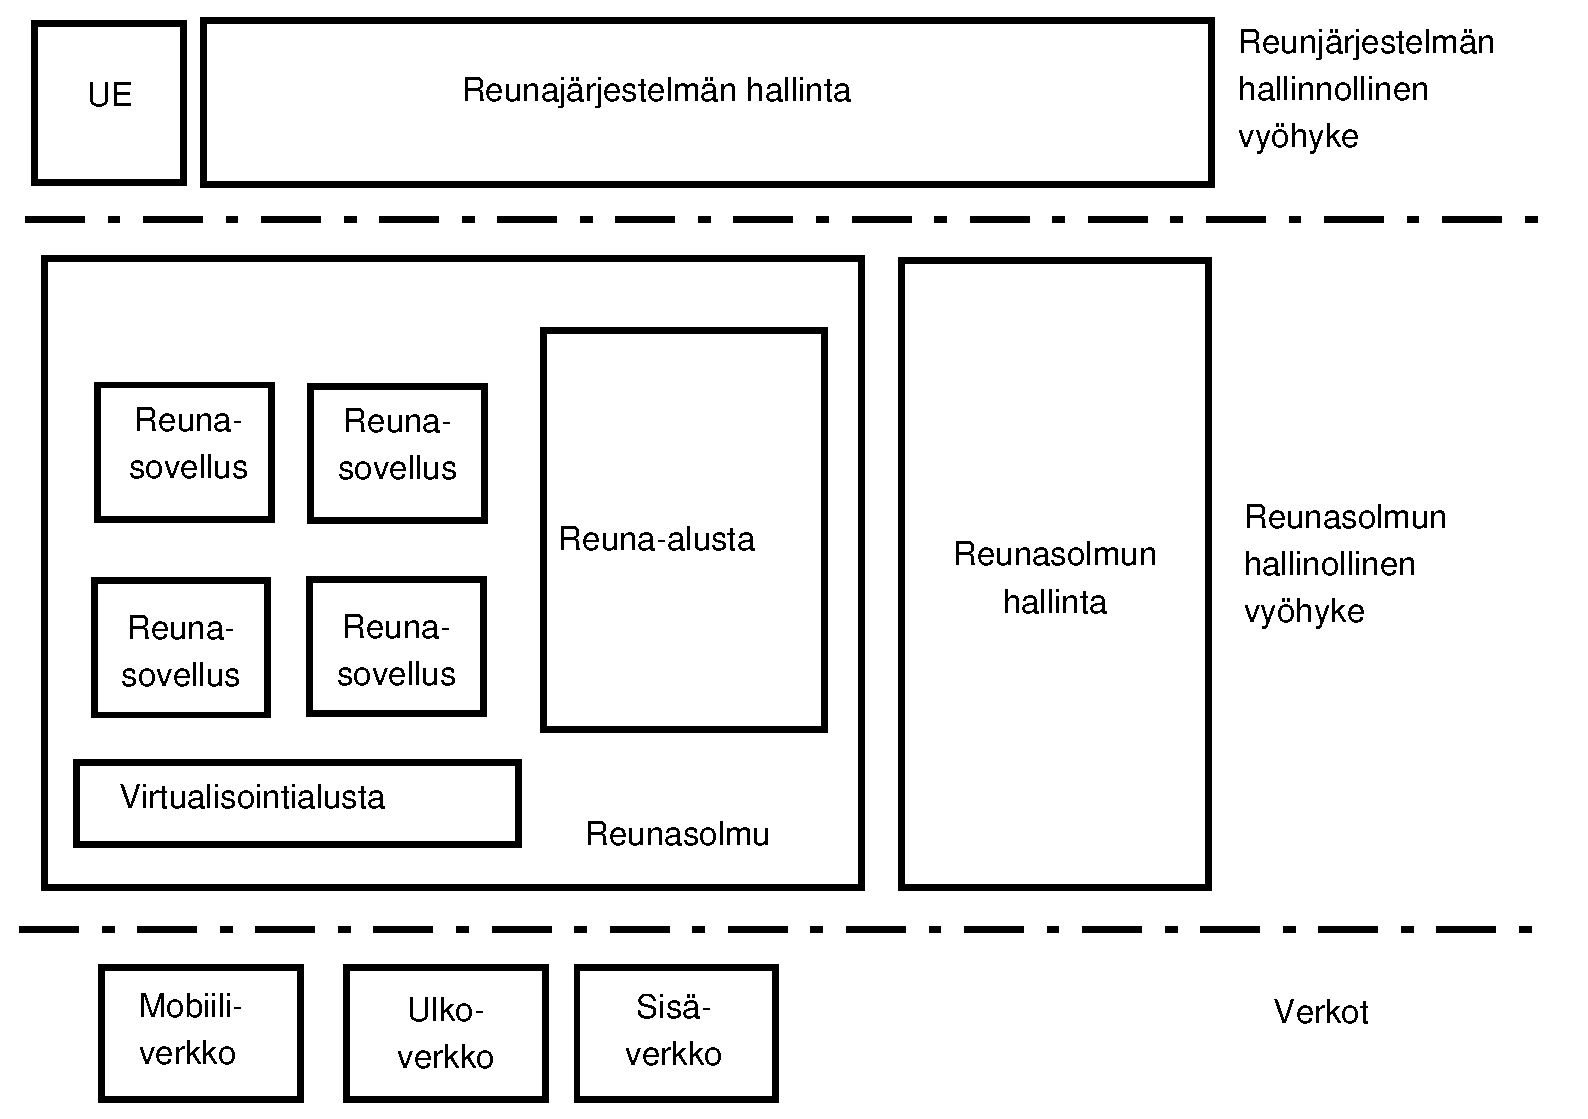
\includegraphics[width = \textwidth]{etsiframework.eps}
\caption{ETSI:n MEC viitekehys \cite{etsirefarch}} \label{fig:etsiframework}
\end{figure}

Referenssiarkkitehtuurissa puolestaan on esitetty funktionaaliset entiteetit. Funktionaalisten entiteettien toiminta on kuvattu.
Referenssiarkkitehtuurissa reunasolmulla (edge host) tarkoitetaan entiteettiä, joka tarjoaa virtualisointi-infrastruktuurin, sekä reunalaskennan toteuttamiseen vaadittavat resurssit (laskenta, tallennus ja verkko).
Reuna-alustalla (Mobile edge platform) tarkoiteen sitä entiteettiä, joka mahdollistaa reunapalveluiden käyttämisen. Reuna-alusta siis mahdollistaa reunapalveluiden saavuttamisen, eli käytännössä tarjoaa rajapinnan asiakaslaitteen suuntaan. Tähän kuuluu siis palvelurekisterin ylläpitäminen, reitityssääntöjen ylläpitäminen, sekä liikenteen välittäminen reunapalveluille. Reuna-alusta voi myös itse tarjota  palveluita.
Esimerkkinä tällaisesta voisi olla tunnistautumispalvelu. 
Reuna-applikaatioilla tarkoitetaan reuna-alustalla suoritettavia virtuaalikoneita, jotka suorittavat reunapalveluiden tuottamiseksi tarkoitettuja ohjelmistoja.

ETSI:n MEC vaatimukset, viitekehys ja referenssiarkkitehtuuri muodostavat puitteet reunajärjestelmän toteuttamiseksi.
Spesifikaatio kuitenkin muovautuu vielä ja muutoksia saattaa tulla. Etenkin NFV:n lopullinen merkitys reunajärjestelmien ja/tai mobiiliverkon toteutuksissa on toistaiseksi avoin kysmys.
